% !TeX program = xelatex
% !BIB program = biber
\documentclass[11pt, a4paper]{article}
\setlength{\marginparwidth}{2cm}
\usepackage[top=2.5cm, bottom=2.5cm, left=2.8cm, right=2.8cm]{geometry}
\usepackage{fontspec}
\usepackage{amsmath}
\usepackage{microtype}
\usepackage{parskip}
\usepackage{graphicx}
\usepackage{float}
\usepackage{booktabs}
\usepackage{listings}
\usepackage{xcolor}
\usepackage{hyperref}
\usepackage{tabularx}
\usepackage{cleveref}
\usepackage[style=ieee, backend=biber]{biblatex}
\usepackage{titling}
\setlength{\droptitle}{-3cm}
\newcolumntype{C}{>{\centering\arraybackslash}X}

\addbibresource{references.bib}

\definecolor{codegray}{RGB}{245,245,245}
\definecolor{codegreen}{RGB}{0,128,0}

\lstset{
    backgroundcolor=\color{codegray},
    basicstyle=\ttfamily\small,
    breaklines=true,
    frame=single,
    framerule=0.4pt,
    rulecolor=\color{gray!40},
    showstringspaces=false,
    commentstyle=\color{codegreen},
}

\hypersetup{colorlinks=true, linkcolor=black, citecolor=black, urlcolor=blue}

\title{\textbf{CSU33D06 Report: Analysis of Headscale}\\
       \large A Self-Hosted Tailscale Control Server}
\author{Xiaoyu SHEN \\ 25369847}
\date{April 2026}

% ──────────────────────────────────────────────────────────────────────────────
\begin{document}

\maketitle
% \tableofcontents
% \newpage

% ══════════════════════════════════════════════════════════════════════════════
\section{Introduction}

Headscale is an open-source, self-hosted re-implementation of the Tailscale control plane, written in Go. It enables individuals and organisations to operate a private WireGuard-based mesh network without depending on Tailscale's commercial infrastructure~\cite{headscale_website_about_faq}. By the date of this report, the project has over $36,177$ GitHub stars, has evolved into widely used infrastructure with a large user community~\cite{headscale_github}.

Headscale is maintained by Kristoffer Dalby and Juan Font ~\cite{headscale_website_welcome}. As documented in the maintainer's own account ~\cite{headscale_FOSDEM2026_speech}, the project began as a small learning experiment intended to understand how Tailscale worked. This trajectory raises a central question for our analysis: \textbf{When an organically grown open-source project scales beyond its original scope without a proportional increase in maintainers or governance structure, what forms of technical and organisational debt emerge, and how are they observable in the codebase?}

To answer this question, this report adopts a data-driven, multi-metric analysis framework that traces the evolution of the project across its lifecycle. Specifically, four complementary metrics are employed to capture different dimensions of technical and organisational debt: \textbf{hotspot concentration} to identify structural bottlenecks in the codebase, \textbf{knowledge concentration} to evaluate the distribution of critical expertise among contributors, \textbf{coordination latency} to measure the cost of cross-author collaboration, and \textbf{mean time to repair} to assess maintenance efficiency and user-facing quality outcomes. In addition, five key stable releases were selected to represent distinct stages in the project's growth trajectory, which will make the analysis more granular and insightful.

% ══════════════════════════════════════════════════════════════════════════════
\section{Why This Project}

% Why you chose it, evidence of complexity and activity.

TCD School of Computer Science and Statistics uses Tailscale as its VPN solution~\cite{TCD_SCSS_support_wiki}, which intrigued me to explore its details. Headscale stood out as a compelling case study for several reasons:
\begin{itemize}
    \item \textbf{Popularity and Activity:} With over 36k stars and 1.5k forks, Headscale has a vibrant community and active development, providing rich data for analysis~\cite{headscale_github}.
    \item \textbf{Technical Complexity:} As a control plane for a mesh VPN, it involves complex networking concepts, state management, and security considerations, making it an interesting subject for software architecture analysis.
    \item \textbf{Organic Growth:} The project evolved from a learning experiment to a widely used tool without a formal governance structure, presenting an opportunity to study the implications of such growth on technical debt and maintainability.
    \item \textbf{My Interest:} As a user of Tailscale and a student who wants to pore over cybersecurity and networking, I want to improve my understanding of this field by analyzing an influential engineering project.
\end{itemize}


% ══════════════════════════════════════════════════════════════════════════════
\section{Stakeholders}
\label{sec:stakeholders}

Following Rozanski and Woods~\cite{R&W_2011}, the stakeholder breakdown below classifies the primary stakeholders identified through analysis of GitHub logs and the keynote address delivered by the project's lead maintainer at FOSDEM 2026~\cite{headscale_FOSDEM2026_speech}. According to this address, the project originated with Juan Font in 2020 during the early COVID-19 period, with Kristoffer Dalby joining as a core contributor in 2021. Following the project's rapid growth in community adoption, Dalby was subsequently hired by Tailscale in 2022, with half his contracted working time formally dedicated to Headscale's continued development.

Unlike projects driven by well-organised teams, structured architecture, and clearly defined roles, Headscale follows a more informal development model. Consequently, its stakeholders' roles are usually fluid and overlapping, and certain roles within Rozanski and Woods' framework~\cite{R&W_2011} remain unfilled or ambiguous. The following stakeholder breakdown and Context View diagram therefore consolidate similar roles and introduce selected "external" components to better capture the project's unique dynamics and interactions.

Entities labelled as External Entity fall outside Rozanski and Woods' stakeholder taxonomy but are included to capture interactions that are material to the system's context and governance dynamics.

\subsection{Juan Font}
\textbf{Role:} Developer, Maintainer, Tester \\
\textbf{Reason:} Founder of Headscale and co-maintainer.

\subsection{Kristoffer Dalby}
\textbf{Role:} Developer, Maintainer, Tester \\
\textbf{Reason:} Lead maintainer of the project.

\subsection{Florian Preinstorfer}
\textbf{Role:} Communicator, Tester \\
\textbf{Reason:} Kristoffer described him as an "excellent documentation writer" who contributes heavily to testing; this is further supported by git log analysis showing substantial documentation and testing contributions.

\subsection{Open-Source Contributors}
\textbf{Role:} Developers \\
\textbf{Reason:} Contribute code through GitHub.

\subsection{Tailscale Inc.}
\textbf{Role:} Supplier \\
\textbf{Reason:} Funds a portion of Kristoffer Dalby's time by employing him, and supplies the protocol and ecosystem upon which Headscale depends. Tailscale engineers maintain active collaboration with the Headscale maintainer, including providing early access to protocol design documents ahead of client releases, ensuring implementation compatibility.

\subsection{Home-Lab or Self-Hoster Users}
\textbf{Role:} Users, Testers, System Administrators, Production Engineers \\
\textbf{Reason:} End users who self-host and maintain private deployments.

\subsection{Enterprise or Corporate Users}
\textbf{Role:} Users, System Administrators, Production Engineers \\
\textbf{Reason:} Some home lab users bring headscale to their organisations, and some companies adopt it to avoid vendor lock-in.

\subsection{Discord Server Members}
\textbf{Role:} Support Staff \\
\textbf{Reason:} Provide community support and discussion in the Discord channel operated by Kristoffer Dalby.

\subsection{GitHub (juanfont/headscale)}
\textbf{Role:} External Entity \\
\textbf{Reason:} Primary platform for source code, issues, pull requests, and release management.

\subsection{OSS Project Adopters}
\textbf{Role:} External Entity \\
\textbf{Reason:} View Headscale as a fallback to reduce vendor lock-in risk. Headscale makes them dare to use Tailscale SaaS.

\subsection{Skeptical Community Members}
\textbf{Role:} External Entity \\
\textbf{Reason:} Concerned about Tailscale's potential embrace-extend-extinguish trajectory and suspect Kristoffer closing issues to protect Tailscale's interest. 

\subsection{Tailscale Client (OSS)}
\textbf{Role:} Supplier \\
\textbf{Reason:} Headscale depends on the debug function or debug feature of the Tailscale client,  which allows kind of overriding the control server. 

\subsection{IonScale / WireFire}
\textbf{Role:} External Entity \\
\textbf{Reason:} Alternative open-source implementations of the Tailscale control server protocol. IonScale explicitly positions itself as a lightweight alternative currently in beta, in contrast to Headscale's goal of full feature parity with Tailscale SaaS. Both projects validate the viability of the open protocol.

\subsection{Tailscale SaaS}
\textbf{Role:} External Entity, Alternative \\
\textbf{Reason:} A proprietary hosted VPN service operated by Tailscale Inc., implementing the same protocol as Headscale. The two are complementary: Headscale serves as an open-source self-hosted alternative.

% ══════════════════════════════════════════════════════════════════════════════
\section{Context View}
\label{sec:context}

The context view in Figure~\ref{fig:context_view} defines the system boundary of Headscale
and its principal external interactions.

\begin{figure}[H]
    \centering
    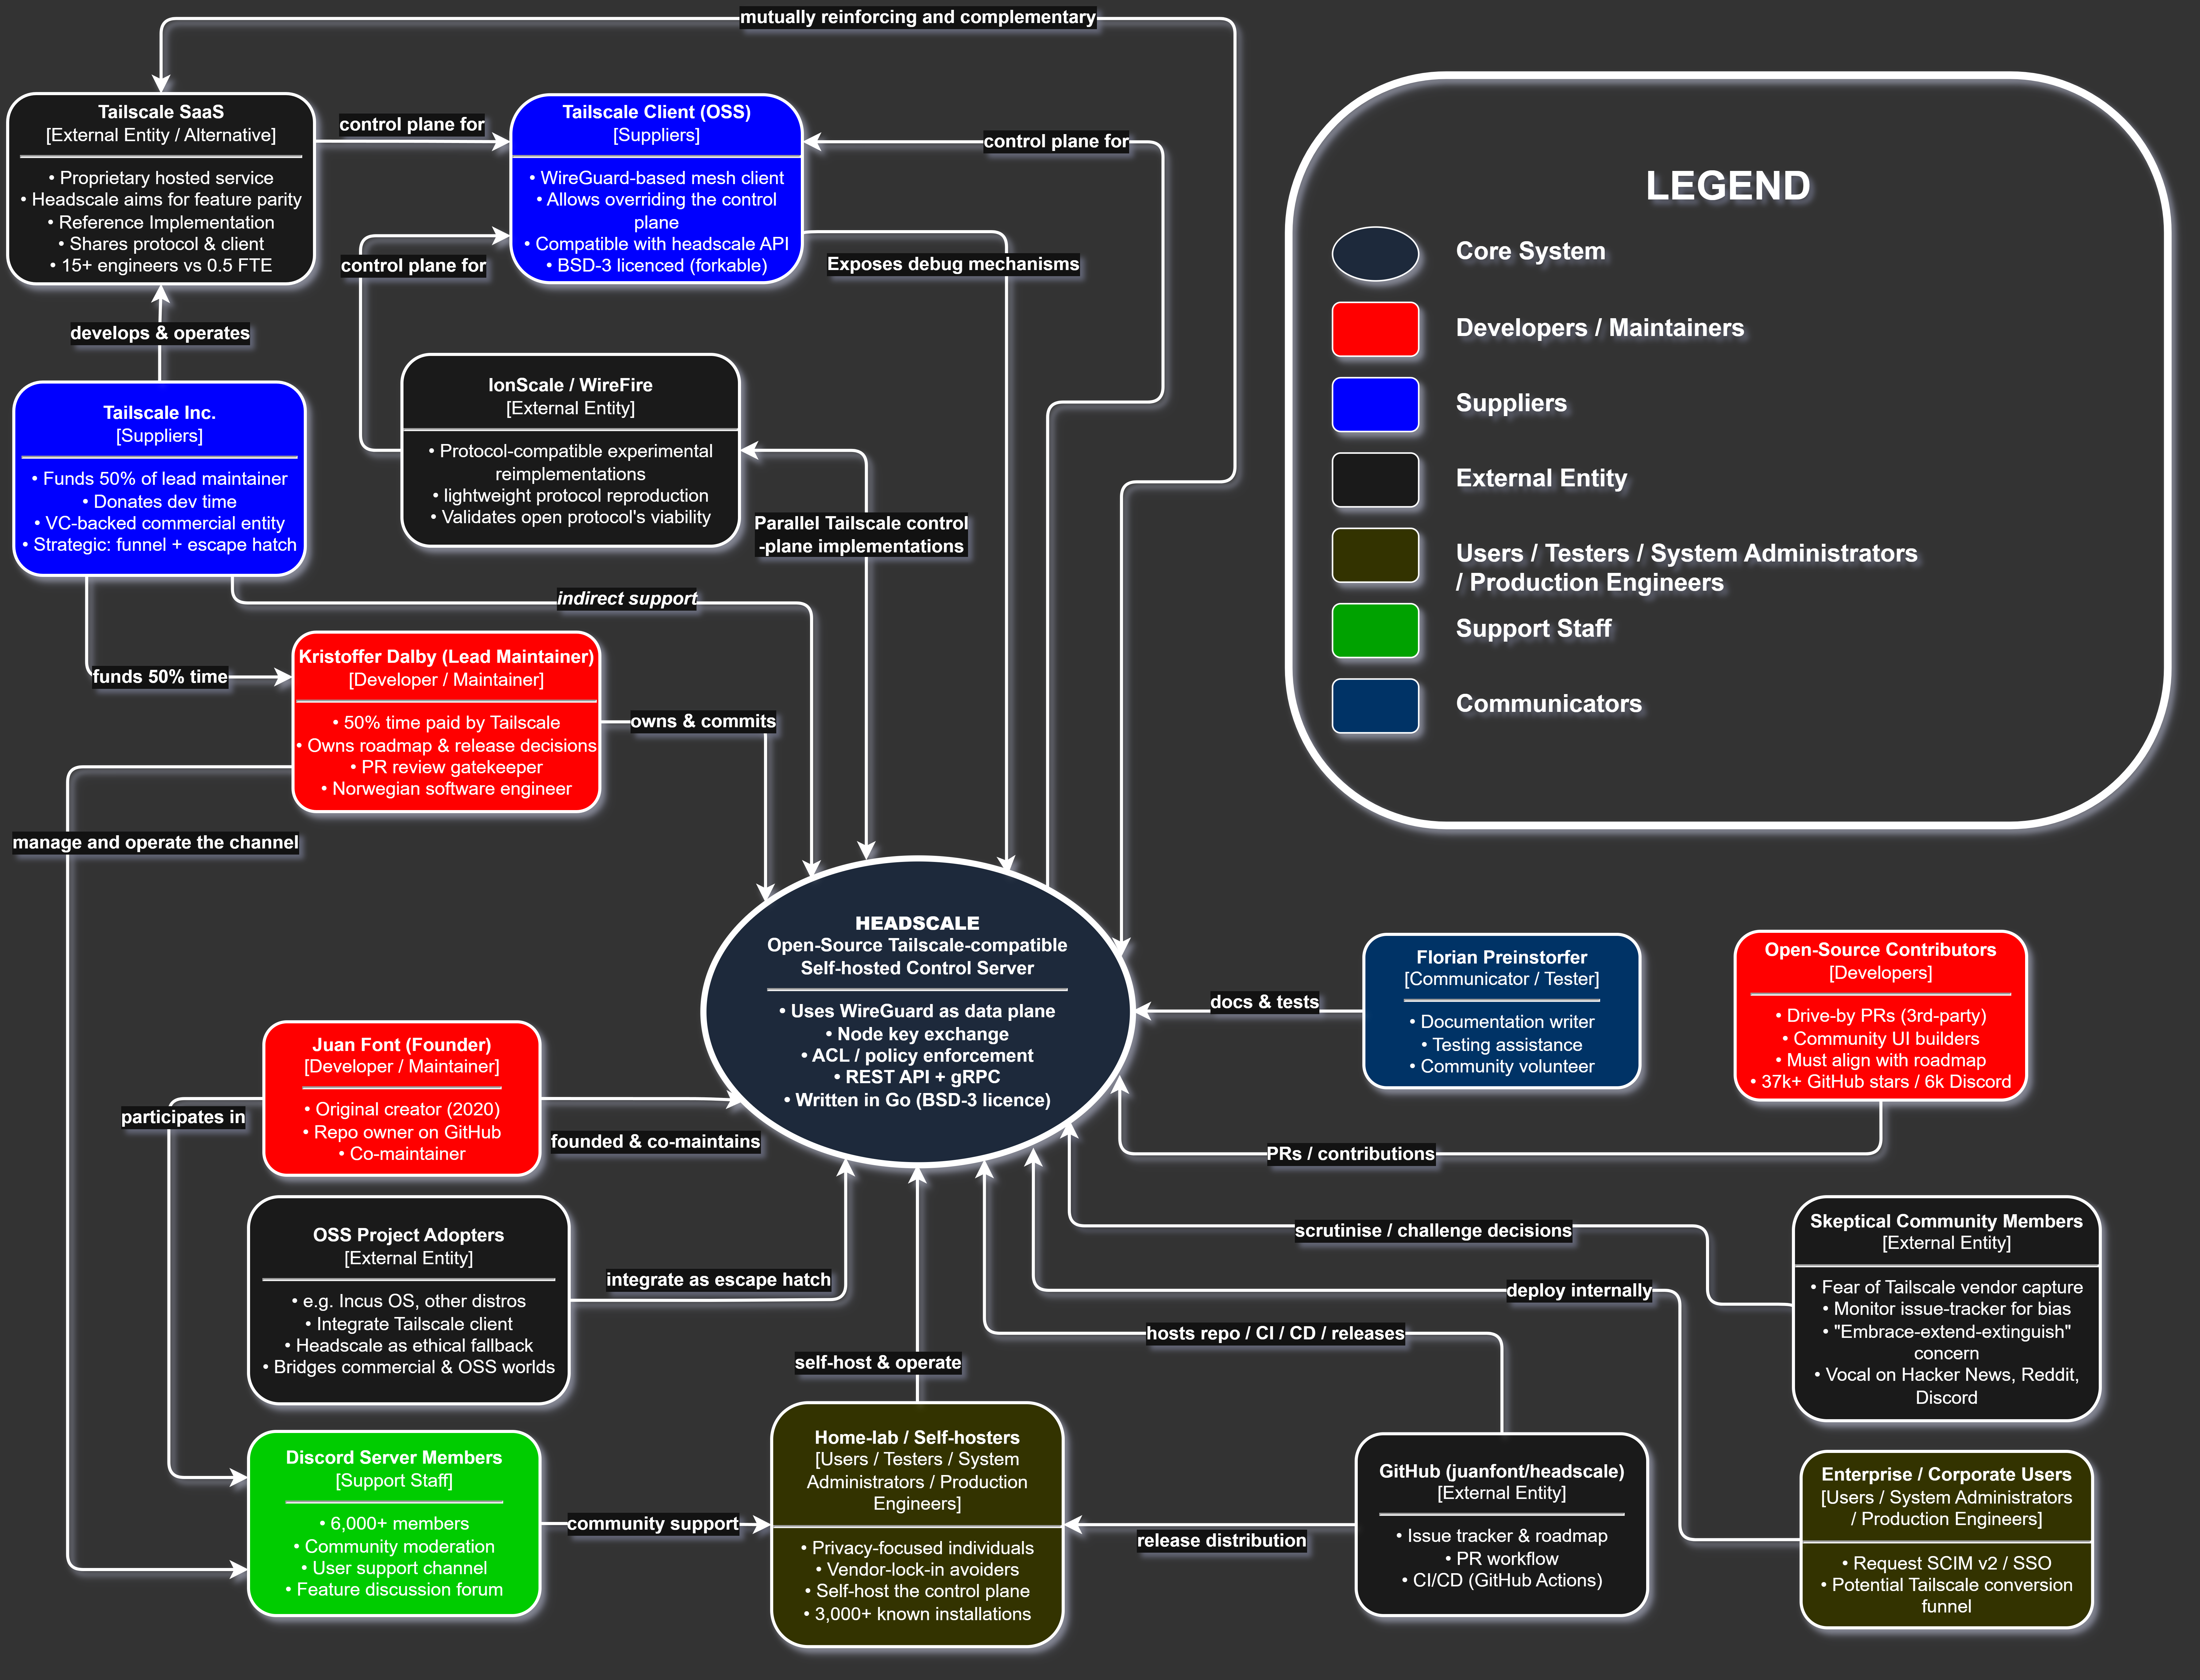
\includegraphics[width=\linewidth]{context_view.png}
    \caption{System context view of Headscale and its external interactions.}
    \label{fig:context_view}
\end{figure}

\paragraph{Tailscale Inc. <--> Headscale}
The most structurally significant external relationship in Headscale's context is the funding arrangement between Tailscale Inc. and its lead maintainer. As Dalby described at FOSDEM 2026~\cite{headscale_FOSDEM2026_speech}, Tailscale Inc. employs him as a software engineer with 50% of his contracted time formally dedicated to Headscale, a deliberate strategic decision by Tailscale to support the open-source ecosystem rather than compete with it. Tailscale's rationale follows a bottom-up marketing model: hobbyists who self-host Headscale may later advocate for Tailscale SaaS adoption in their organisations, making Headscale a de facto indirect acquisition channel. Beyond funding, the relationship also provides Headscale with early access to Tailscale's internal protocol design documents ahead of client releases, enabling the project to maintain compatibility with upstream changes. This arrangement, however, introduces a structural tension: any roadmap or triaging decision made by Dalby is subject to scrutiny from community members who suspect bias toward Tailscale's commercial interests. Dalby himself acknowledged this dynamic directly, recounting an incident in which routine issue-tracker grooming was publicly interpreted as deliberate suppression of features that would compete with Tailscale SaaS~\cite{headscale_FOSDEM2026_speech}. The governance structure does provide a nominal separation — Dalby's contributions flow through a personal fork before being merged into the canonical repository owned by Juan Font — but this remains an informal safeguard rather than a formal governance mechanism.

\paragraph{Tailscale Client --> Headscale}
Headscale's operation depends on a debug feature in the open-source Tailscale client that allows the control server endpoint to be overridden. While Dalby acknowledged this could theoretically be removed~\cite{headscale_FOSDEM2026_speech}, he noted that the client is BSD-3 licensed and therefore forkable, providing a meaningful fallback. This dependency is therefore better characterised as a protocol-compatibility constraint than a critical vulnerability: so long as the open-source client remains forkable, the community retains the ability to maintain a compatible client independently.

\paragraph{Tailscale SaaS <--> Headscale}
Headscale positions itself as complementary to rather than competitive with Tailscale SaaS, implementing the same protocol and aiming for feature parity with the hosted service. However, the relationship is fundamentally asymmetric: Tailscale SaaS is developed by a team of over 15 engineers, while Headscale is maintained by the equivalent of 0.5 full-time employees~\cite{headscale_FOSDEM2026_speech}. Dalby described the practical implication clearly — full feature parity is not a realistic near-term goal, and the gap is not merely a matter of velocity but of structural capacity. Tailscale SaaS thus acts as both the reference implementation and an implicit ceiling on Headscale's roadmap ambitions. The protocol design documents shared by Tailscale engineers in advance of client releases partially mitigate this asymmetry at the protocol level, but at the product level the disparity remains a defining constraint on the project's development trajectory.

\paragraph{Enterprise Users --> Headscale --> Tailscale SaaS}
A particularly notable interaction pattern involves enterprise and OSS-project adopters who use Headscale not primarily as an active deployment but as a strategic escape hatch. As Dalby explained, users who might otherwise be reluctant to depend on a proprietary SaaS become willing to adopt Tailscale precisely because Headscale exists as a self-hosted fallback — should Tailscale's commercial terms or availability change, a migration path remains open~\cite{headscale_FOSDEM2026_speech}. He cited the Incus OS project as a concrete example: its maintainer explicitly justified integrating Tailscale client support on the grounds that Headscale compatibility preserved the project's open-source ethos. This dynamic means Headscale simultaneously reduces vendor lock-in risk for its users and, paradoxically, expands Tailscale's addressable market by making the commercial product more palatable to lock-in-sensitive adopters. From Tailscale Inc.'s perspective, Headscale functions both as a community goodwill signal and as an indirect sales enabler — a dual role that further explains the company's willingness to fund its development.

\paragraph{Reflection}
The stakeholder analysis relies heavily on a single primary source — the lead maintainer's FOSDEM 2026 keynote~\cite{headscale_FOSDEM2026_speech} — with limited triangulation from independent sources, which may introduce perspective bias. While supplementary signals were gathered from GitHub activity and community discussions on Discord, these sources are informal and indirect in nature and therefore cannot be considered strong standalone evidence for validating the findings.

% ══════════════════════════════════════════════════════════════════════════════
\section{Software Metrics}
\label{sec:metrics}

\subsection{Metric Selection}

To reveal the technical debt and maintainability challenges as the project scaled without a proportional increase in maintainers or governance structure, four metrics were selected to probe different quality dimensions:

\begin{enumerate}
    \item \textbf{Hotspot Risk}: Given that Headscale originated from informal development, early core files may have gradually accumulated complexity and potential design antipatterns. This metric helps identify whether these files continue to act as structural bottlenecks, potentially constraining future refactoring and feature development.
    \item \textbf{Knowledge Concentration}: As the project is driven by a small number of core developers, critical implementation knowledge may remain centralized even as the development team expands. This metric assesses whether community growth has successfully distributed that knowledge.
    \item \textbf{Coordination Latency}: Informal projects lack efficient structures. This metric reflects whether the lack of structure leads to increasing coordination overhead as the project scales.
    \item \textbf{Mean Time to Repair}: This metric reflects the robustness of the project's maintenance capacity and how community growth influences the bug resolution process, indicating whether maintenance efficiency scales effectively with project growth.
\end{enumerate}
\label{item:metrics}

\subsection{Stage Window Definition}

To better understand the project's evolution, the metric analysis uses a hybrid windowing strategy. M1 and M2 use cumulative windows (Start $\rightarrow$ current stage) to capture the accumulation of technical debt, while M3 and M4 use segmented windows (previous stage $\rightarrow$ current stage) to evaluate friction in each stage. For cumulative windows, the start release version v0.1.0 is used as the lower bound.

\begin{table}[H]
\centering
\small
\begin{tabularx}{\textwidth}{|C|C|C|C|C|}
    \hline
    \textbf{Stage} & \textbf{Version} & \textbf{Date} & \textbf{Cumulative Range (M1/M2)} & \textbf{Segmented Range (M3/M4)} \\
    \hline
    Start & v0.1.0 & 2021-06-14 & v0.1.0 & v0.1.0 \\
    \hline
    Early growth & v0.12.1 & 2021-12-24 & v0.1.0-v0.12.1 & v0.1.0-v0.12.1 \\
    \hline
    Expansion & v0.17.1 & 2022-12-05 & v0.1.0-v0.17.1 & v0.12.1-v0.17.1 \\
    \hline
    Maturity & v0.22.3 & 2023-05-12 & v0.1.0-v0.22.3 & v0.17.1-v0.22.3 \\
    \hline
    Current & v0.28.0 & 2026-02-04 & v0.1.0-v0.28.0 & v0.22.3-v0.28.0 \\
    \hline
\end{tabularx}
\caption{Selected stable releases and window definition used for metric computation.}
\label{tab:window_definition}
\end{table}


\subsection{Static Analysis}

The Herfindahl--Hirschman Index (HHI), originally developed as a market concentration measure in economics~\cite{tung_truong_integrated_2021}, is here adapted as a general-purpose concentration metric to quantify the distribution of file churn across the codebase.

\[
\text{HHI} = \sum_i s_i^2,
\]
where $s_i$ is the touch-event share of file $i$ in the corresponding window.

\subsubsection{M1 Hotspot Concentration (HHI)}

M1 uses file churn concentration to identify structural hotspots across release windows. Lower HHI and lower Top10 share indicate better distribution of change across the codebase, while higher values suggest concentration in a few files.

\begin{table}[H]
\centering
\small
\begin{tabularx}{\textwidth}{|C|C|C|C|C|C|}
    \hline
    \textbf{Stage} & \textbf{Touch Events} & \textbf{Top10 Share (\%)} & \textbf{Top1 Share (\%)} & \textbf{HHI} & \textbf{Top 3 Hotspots} \\
    \hline
    Start & 313 & 51.12 & 9.27 & 0.0376 & \path{cmd/headscale/headscale.go}; \path{README.md}; \path{api.go} \\
    \hline
    Early growth & 1322 & 40.47 & 6.35 & 0.0238 & \path{app.go}; \path{api.go}; \path{machine.go} \\
    \hline
    Expansion & 3455 & 31.43 & 5.62 & 0.0164 & \path{app.go}; \path{machine.go}; \path{api.go} \\
    \hline
    Maturity & 4436 & 27.28 & 4.62 & 0.0129 & \path{app.go}; \path{machine.go}; \path{CHANGELOG.md} \\
    \hline
    Current & 9314 & 16.89 & 3.47 & 0.0059 & \path{CHANGELOG.md}; \path{app.go}; \path{machine.go} \\
    \hline
\end{tabularx}
\caption{M1 Hotspot Concentration by stage.}
\label{tab:m1_hotspot_risk}
\end{table}

The concentration of churn declines over the full history (Top10 share from 51.12\% to 16.89\%, HHI from 0.0376 to 0.0059), suggesting broader change distribution. However, recurring core files remain visible hotspots across phases. This twist may suggest a redistribution of change pressure rather than its elimination. The project still relies on a small set of critical files that may accumulate technical debt without proper attention.
In addition, notice that the CHANGELOG.md file becomes a hotspot in later stages, suggesting that documentation churn is absorbing a portion of the measured hotspot pressure, which may mask underlying code-level concentration.


\subsubsection{M2 Knowledge Concentration}

M2 evaluates authorship concentration at commit level. Lower HHI and higher Bus Factor ~\cite{bus_factor} indicate better knowledge distribution.

\begin{table}[H]
\centering
\small
\resizebox{\textwidth}{!}{%
\begin{tabularx}{\textwidth}{|C|C|C|C|C|C|C|C|}
    \hline
    \textbf{Stage} & \textbf{Commits} & \textbf{Authors} & \textbf{Top1 Share (\%)} & \textbf{Top2 Share (\%)} & \textbf{HHI} & \textbf{Effective Authors} & \textbf{Bus Factor 50} \\
    \hline
    Start & 121 & 7 & 74.38 & 90.08 & 0.5825 & 1.72 & 1 \\
    \hline
    Early growth & 611 & 32 & 50.57 & 68.74 & 0.3114 & 3.21 & 1 \\
    \hline
    Expansion & 1740 & 96 & 42.87 & 64.37 & 0.2419 & 4.13 & 2 \\
    \hline
    Maturity & 2005 & 130 & 42.69 & 61.40 & 0.2333 & 4.29 & 2 \\
    \hline
    Current & 2803 & 238 & 48.16 & 61.54 & 0.2602 & 3.84 & 2 \\
    \hline
\end{tabularx}%
}
\caption{M2 Knowledge Concentration by stage.}
\label{tab:m2_knowledge_concentration}
\end{table}

According to the tendency of the data, a structural twist is observed in the knowledge concentration pattern: knowledge concentration weakens through Maturity, then re-concentrates in Current (Top1 share rises from 42.69\% to 48.16\% and HHI from 0.2333 to 0.2602) while the total author count keeps rising. This phenomenon may indicate that among the 238 authors, the vast majority belong to the long tail of low-frequency contributors, and the core developers still play a significant role. This conclusion is consistent with the BusFactor 50 result, which is stable across all stages.

\subsection{Dynamic Analysis}

\subsubsection{M3 Coordination Latency}

M3 tracks cross-author handoff dynamics on the same file, where latency is measured as the median delay between adjacent edits by different authors. This operationalisation is inspired by socio-technical congruence research, where coordination requirements arise from task dependencies between developers ~\cite{cataldo_coordination_2013}, and delays in recognising or addressing these coordination needs can negatively impact collaboration efficiency ~\cite{blincoe_proximity_2012}.

\begin{table}[H]
\centering
\small
\begin{tabularx}{\textwidth}{|C|C|C|C|}
    \hline
    \textbf{Stage} & \textbf{Handoff Rate (\%)} & \textbf{Median Handoff (days)} & \textbf{P75 Handoff (days)} \\
    \hline
    Start & 23.98 & 4.04 & 13.37 \\
    \hline
    Early growth & 30.44 & 6.30 & 20.23 \\
    \hline
    Expansion & 42.22 & 9.37 & 26.78 \\
    \hline
    Maturity & 34.08 & 15.31 & 43.57 \\
    \hline
    Current & 32.49 & 21.27 & 60.08 \\
    \hline
\end{tabularx}
\caption{M3 Coordination Latency by stage.}
\label{tab:m3_coordination_latency}
\end{table}

Coordination overhead grows over time: while handoff rate peaks in the middle of the period, handoff delay rises substantially. This internal divergence within the metric may suggest that code ownership patterns are emerging. Considering the knowledge concentration pattern in M2, this phenomenon may be the observable manifestation of accumulated organisational technical debt, expressed as increasing time overhead.

\subsubsection{M4 Mean Time to Repair}

M4 employs two complementary sub-measurements (M4A and M4B) to mitigate the limitations of each individual proxy:

\paragraph{M4A File-Touch Proxy}
For each fix-related commit in segmented windows, M4A is measured as the delay between the fix commit timestamp and the latest previous touch timestamp on any changed file. This metric serves as a proxy for repair latency, inspired by defect resolution time analyses in mining software repositories literature~\cite{kim_defect_resolution_time_2006}. While conceptually related to Mean Time to Repair (MTTR), which measures the time required to restore a system after failure~\cite{perry_testing_reliability}, this study operationalises repair latency at the file and commit level.

\begin{table}[H]
\centering
\small
\begin{tabularx}{\textwidth}{|C|C|C|C|C|}
    \hline
    \textbf{Stage} & \textbf{Samples} & \textbf{Mean (days)} & \textbf{Median (days)} & \textbf{P75 (days)} \\
    \hline
    Start & 11 & 8.17 & 0.81 & 8.44 \\
    \hline
    Early growth & 93 & 3.12 & 0.86 & 3.19 \\
    \hline
    Expansion & 156 & 8.36 & 0.76 & 8.45 \\
    \hline
    Maturity & 20 & 15.38 & 2.22 & 24.91 \\
    \hline
    Current & 122 & 19.49 & 5.05 & 19.22 \\
    \hline
\end{tabularx}
\caption{M4A File-Touch Proxy MTTR by stage.}
\label{tab:m4a_mttr_file_touch}
\end{table}

\paragraph{M4B Bug-Only Issues}
Given that this repository includes many feature requests issues, only bug fix issues are included in M4B to better capture the Mean Time to Repair (MTTR). For each closed bug-labeled issue in \texttt{juanfont/headscale}, M4B is measured as the time difference between \texttt{closed\_at} and \texttt{created\_at}.

\begin{table}[H]
\centering
\small
\begin{tabularx}{\textwidth}{|C|C|C|C|C|}
    \hline
    \textbf{Stage} & \textbf{Samples} & \textbf{Mean (days)} & \textbf{Median (days)} & \textbf{P75 (days)} \\
    \hline
    Start  & 0 & N/A & N/A & N/A \\
    \hline
    Early growth & 5 & 16.00 & 6.87 & 27.91 \\
    \hline
    Expansion & 103 & 31.86 & 5.60 & 43.17 \\
    \hline
    Maturity & 74 & 64.17 & 12.92 & 82.84 \\
    \hline
    Current & 479 & 81.12 & 20.05 & 102.22 \\
    \hline
\end{tabularx}
\caption{M4B Bug-Only Issue MTTR by stage}
\label{tab:m4b_mttr_bug_issues}
\end{table}

The high mean and low median in M4A suggest a long-tail distribution of repair times, likely attributable to a small number of structurally complex, high-coupling files.

M4B shows a long-tail repair profile in the live dataset (overall median 13.84 days, P90 205.41 days), with stage-level median MTTR rising from 6.87 days in Early growth to 20.05 days in Current. Moreover, the mean MTTR rises more substantially (16.00 days to 81.12 days), which may reflect that the tech debt in current stage impacts the user's experience and confidence in the project robustness. 

\subsection{Metric Summary and Reflection}

\paragraph{Summary}
Holistically considering all the four metrics, the analysis reveals a general picture of Headscale's technical debt evolution. In Phase 1 (Start to Early Growth), the project is characterized by strong founder dependency, with a single dominant contributor (Bus Factor 50 = 1) and highly concentrated code hotspots in core logic. During this stage, mean time to repair (MTTR) remains low due to minimal decision latency, as the founder directly resolves issues. This pattern reflects a form of “productive” or “benign” technical debt, representing a necessary trade-off for rapid iteration. In Phase 2 (Expansion to Maturity), the number of contributors increases and the Herfindahl–Hirschman Index (HHI) declines, suggesting a superficially healthier distribution of contributions. However, coordination latency begins to rise significantly, and MTTR exhibits increasing variance. Simultaneously, code hotspots expand beyond core logic into peripheral artifacts such as changelog files, indicating a shift in system activity. At this stage, technical debt transitions from a purely technical phenomenon to an organizational one. In Phase 3 (Current), the project enters a scaling crisis marked by the simultaneous deterioration of multiple indicators: knowledge concentration as measured by M2 HHI rebounds, coordination delay (M3, P75) reaches 60 days, mean MTTR for bug-related issues (M4B) rises to 81 days, and the bug sample size expands to 479. A pronounced disparity emerges between the nominal contributor base (238 authors) and the effective decision-making core (Bus Factor 50 = 2), revealing a widening governance gap. Collectively, these patterns point to a typical open-source failure mode~\cite{coelho_why_2017} in which apparent popularity and growth mask an underlying loss of coordination efficiency and an erosion of project control.

\textbf{Reflection}
\begin{itemize}
    \item For M3: Cross-author file transitions are treated as a proxy for coordination overhead; however, such transitions may also reflect independent ownership shifts rather than active collaboration handoffs.
    \item For M4A: M4A measures the elapsed time since the most recent modification to affected files, which serves as a proxy for repair latency rather than a direct measure of fault introduction–to–resolution interval. The heuristic keyword-based identification of fix-related commits introduces noise, as the pattern may both miss synonymous terms and include false positives such as error-handling refactors.
\end{itemize}



% ══════════════════════════════════════════════════════════════════════════════
\section{Conclusion}

The data provides clear answers for the research question and reveals the typical technical debt evolution pattern in an organically grown open-source project. Technical debt initially manifests as a concentration of code hotspots ~\cref{tab:m1_hotspot_risk}, and appears to dissipate as the codebase expands. However, knowledge debt persists over time and resurges during later stages of scaling ~\cref{tab:m2_knowledge_concentration}, constituting the most structurally significant risk within the project. Coordination debt, in contrast, grows monotonically with increasing project complexity, manifesting as the time overhead imposed by organisational inefficiencies ~\cref{tab:m3_coordination_latency}. Finally, quality debt can be viewed as the cumulative outcome of these preceding forms of debt: although it emerges at a later stage, it exerts the most tangible impact on end users ~\cref{tab:m4a_mttr_file_touch} \& ~\cref{tab:m4b_mttr_bug_issues}. It is reasonable to assume that such a pattern is not unique to Headscale, but rather reflects a common trajectory for organically grown open-source projects, consistent with findings in the literature~\cite{coelho_why_2017}. 


\newpage
\printbibliography[heading=bibintoc]

\end{document}